\documentclass[10pt]{article}

\usepackage{jmlr2e}
\usepackage{natbib}
\usepackage{hyperref}
\usepackage{amssymb,amsmath,epsfig}
\usepackage{caption}
\usepackage[utf8]{inputenc}
\usepackage[french]{babel}
\usepackage{lipsum}
\usepackage{datenumber}
\usepackage{float}
\usepackage[T1]{fontenc} % Add this line for T1 encoding
\usepackage[utf8]{inputenc} % This line is for input encoding, usually utf8
\usepackage[french]{babel} % Your existing line for French language support

\sloppy

\renewcommand{\rmdefault}{ptm} % Changes font to Times
%%%%%%%%%%%%%%%%%%%%%%%

\newcounter{prevyear}
\setmydatenumber{prevyear}{\the\year}{1}{1}
\addtocounter{prevyear}{-1}


%\editor{Machine Learning Avancé (2021-2022)}

\begin{document}

\title{Data-Free Quantization\\
Through Weight Equalization and Bias Correction}
\editor{Machine Learning Avancé (\theprevyear-\the\year)}

%% Group authors per affiliation:

\author{\name Djamai Hania \email Hania.Djamai@etu.sorbonne-universite.fr
       \AND
       \name Amroun Abdelkader \email Abdelkader.Amroun@etu.sorbonne-universite.fr
       \AND
       \name Mahfoudi Assil \email Assil.Mahfoudi@etu.sorbonne-universite.fr
       \AND
       \name Saïdani Nidhal \email ns+su@pm.me}

\newcommand{\addr}[1]{\noindent\textbf{Master Ingénierie des Systèmes Intelligents \\ 
Sorbonne Université \\ 
Paris, France}}

\addr

\maketitle

% Abstract section

\begin{abstract}

\textbf{Le résumé  synthétise en environ 200 mots la tâche abordées, les problèmes associés, la solution proposée, et les résultats principaux} \\

This report delves into the implementation of quantization techniques aimed at optimizing Deep Neural Networks (DNNs) for enhanced inference performance. By quantizing neural network models, we effectively reduce their storage footprint and leverage integer arithmetic for faster computation, capitalizing on the integer math pipelines of modern processors. We present a comprehensive review of the mathematical underpinnings of quantization parameters and their impact on a diverse set of DNN architectures across various domains such as image processing, speech recognition, and natural language processing. Special emphasis is placed on quantization approaches that seamlessly integrate with and exploit the capabilities of high-throughput integer units, thus facilitating efficient hardware acceleration. Through a series of experiments, we assess the influence of different quantization strategies on model accuracy and computational efficiency, offering insights into their practical applicability. Our findings suggest that intelligent quantization can significantly expedite DNN inference without compromising on model fidelity, thereby serving as a pivotal step towards deploying AI in resource-constrained environments.
\end{abstract}

\begin{keywords}
Data-free quantization, Bias correction, 8-bit fixed-point quantization, Deep neural networks
\end{keywords}


\section{Introduction}
\lipsum[1]
\section{Partie Amroun/Mahfoudi}
\lipsum[1]

\section{Quantization Bias Correction in Neural Networks}

Deep Learning models are increasingly focusing on efficiency, balancing precision with model compactness in response to the growing demands of modern applications. At the forefront of this transformative shift is quantization, a technique that reduces model size and enhances inference speed by converting the precision of weights and activations from FLOAT32 to INT8.\\

Post-Training Quantization (PTQ) epitomizes this transformation, allowing pre-trained neural networks to be converted into fixed-point representations without retraining or access to the original training data. This approach meticulously calibrates weights and quantization parameters to optimize model performance. Within PTQ, 'Quantization Bias Correction' emerges as a crucial component to preserve the predictive accuracy of models. Quantization can introduce biases, skewing activation values and potentially causing significant deviations from the intended outputs of the model.\\

Our report delves into advanced data-free quantization techniques, such as Cross-Layer Range Equalization and High-Bias Absorption, to address these challenges. These techniques are indispensable in achieving the delicate balance between compactness and accuracy in lightweight models.\\

The workflow begins with a pre-trained floating-point model. The process initiates with Cross-Layer Equalization (CLE), which standardizes weight ranges across layers, thereby facilitating uniform quantization. This is followed by the introduction of quantizers and precise adjustments to weight ranges. In scenarios with available data, methods like AdaRound and Bias Correction are employed to fine-tune the quantization process. In contrast, data-scarce environments benefit from Batch Normalization (BN) based range adjustment, offering a robust, data-independent alternative.\\

Our analysis aims to illuminate these methodologies, highlighting their effectiveness in preserving the behavior of the original model post-quantization. As a fundamental technique in model compression and acceleration, quantization is pivotal for reducing model size and enhancing inference speed, achieving these objectives with minimal accuracy loss.

\subsection{Overview of Neural Network Quantization}

Neural network quantization is a pivotal process for enhancing computational efficiency in machine learning. It involves converting floating-point representations, typically FP32, to lower bit-width formats like INT8. This reduction is crucial for optimizing neural network (NN) accelerators, which perform core operations like matrix-vector multiplications.

\subsubsection{Quantize Bias Correction in DFQ}

A critical aspect of DFQ is the Quantize Bias Correction. This process aims to rectify the biases that arise during the quantization of neural networks. Quantization, while reducing model size and enhancing computational efficiency, can inadvertently skew activation values. These deviations can significantly impact the model's predictive accuracy.

Bias Correction in DFQ involves adjusting these biases to align the quantized model's behavior closely with its original, high-precision counterpart. This step is crucial for maintaining accuracy, especially when transitioning from high-precision formats like FP32 to lower-precision, such as INT8, without access to the original training dataset. By fine-tuning the biases in the quantization process, DFQ ensures that the efficiency gains from model compression do not come at the cost of performance degradation.

This balanced approach in DFQ, particularly through Quantize Bias Correction, provides a robust solution for deploying efficient and accurate neural network models in data-sensitive environments.

\subsection{Implementing Analytical Bias Correction}

\subsubsection{Background}
In our implementation, we focus on the "Analytical Bias Correction" method as outlined in the paper by Nagel et al. (2019). This technique is particularly relevant for neural networks that utilize batch normalization and ReLU activations, aiming to correct biased errors caused by quantization analytically.

\subsubsection{Approach}
The implementation involves several key steps:

\begin{enumerate}
    \item \textbf{Statistical Analysis of Batch Normalization Layer:} Analyze the batch normalization (BN) statistics, extracting the scale (\(\gamma\)) and shift (\(\beta\)) parameters, which are crucial for estimating the input distribution.
    \item \textbf{Estimation of Input Distribution:} Use the BN statistics to estimate the expected input distribution, forming the basis for the bias correction calculation.
    \item \textbf{Calculation of Bias Correction Term:} Calculate the bias correction term based on the estimated input distribution, aligning the quantized model output with the original FP32 model.
    \item \textbf{Integration into the Model:} Integrate the bias correction term into the model, adjusting the bias parameter of relevant layers to align with the original model's performance.
\end{enumerate}

\subsubsection{Practical Considerations}
\begin{itemize}
    \item \textbf{Data Independence:} This method is independent of the original training data, making it suitable for scenarios with data privacy or accessibility concerns.
    \item \textbf{Compatibility with Network Architectures:} The method is broadly applicable but most effective in networks with significant reliance on batch normalization and ReLU activations.
    \item \textbf{Performance Evaluation:} After implementation, assess the accuracy of the quantized model against the original FP32 model to ensure effective bias correction.
\end{itemize}

%%%
\subsection{Fixed-Point Quantization}

Fixed-point quantization in Quantized Neural Networks (QNNs) is a key technique for reducing computational complexity while preserving accuracy. This subsection explores two primary quantization strategies: Symmetric and Asymmetric Quantization, followed by an examination of the quantization schematic in convolutional layers.

\subsubsection{Symmetric Quantization}

Symmetric Quantization directly maps the absolute maximum value of the floating-point range to the fixed-point range, keeping the zero point's alignment. The scaling factor in this method is crucial and is defined as:

\begin{equation}
    qx = \frac{(2^n - 1) / 2}{2 \times \max(\left| xf \right|)}
\end{equation}

Here, \( n \) represents the bit width of the fixed-point data type. The quantized value in the integer range is obtained by:

\begin{equation}
    xq = \text{round}(qx \times xf)
\end{equation}

\begin{figure}[H]
\centering
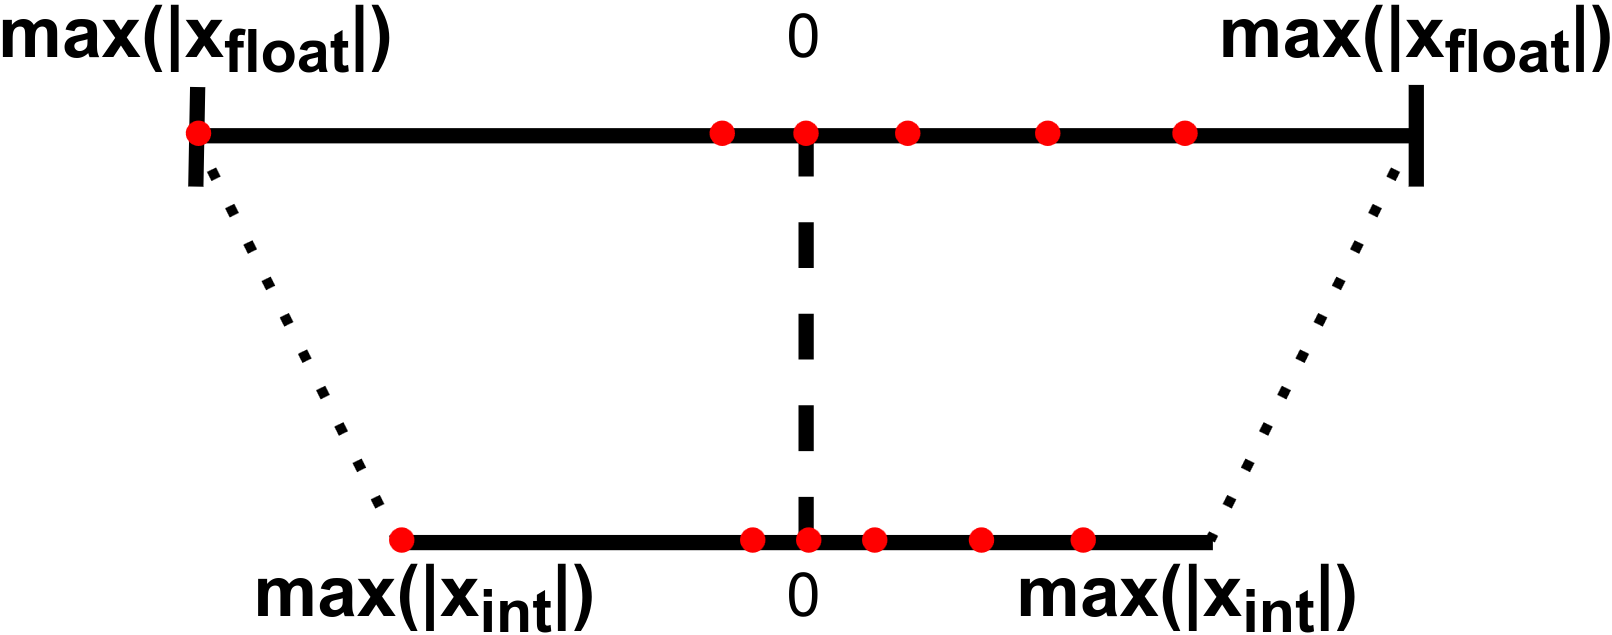
\includegraphics[width=0.5\textwidth]{figures/symmetric_quant.png}
\caption{Illustration of Symmetric Quantization}
\label{fig:symmetric_quantization}
\end{figure}

Refer to Figure~\ref{fig:symmetric_quantization} for a visual representation of Symmetric Quantization.

\subsubsection{Asymmetric Quantization}

Asymmetric Quantization introduces a quantization bias or offset, allowing for an adjusted mapping of the min/max floating-point range to the integer range. The quantization formula incorporating this bias is given by:

\begin{equation}
    qx = \text{scale factor}
\end{equation}
\begin{equation}
    xq = \text{round}(qx \times (xf - \text{bias}))
\end{equation}

\begin{figure}[H]
\centering
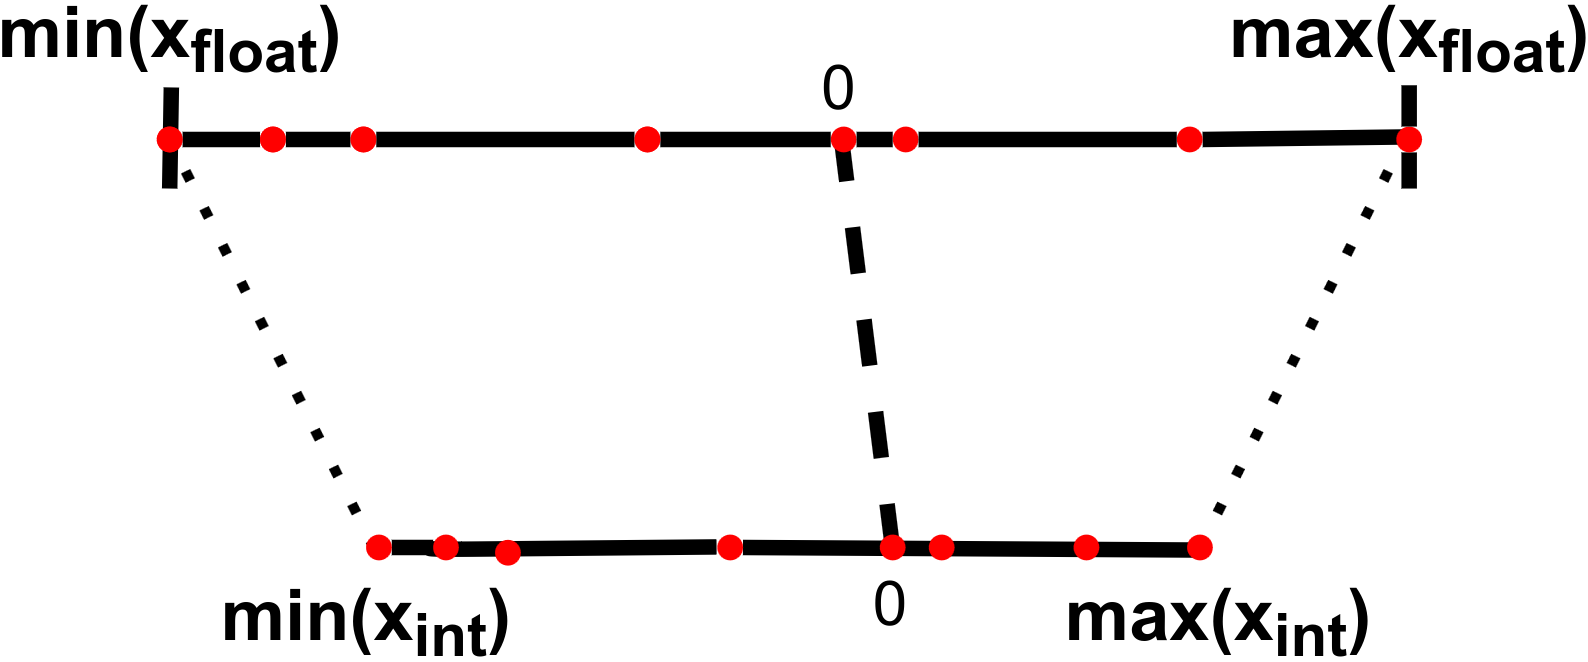
\includegraphics[width=0.5\textwidth]{figures/asymmetric_quant.png}
\caption{Illustration of Asymmetric Quantization}
\label{fig:asymmetric_quantization}
\end{figure}

Figure~\ref{fig:asymmetric_quantization} demonstrates Asymmetric Quantization.

\subsubsection{Quantization Schematic of a Convolutional Layer}

The quantization schematic of a convolutional layer, particularly for 8-bit and 32-bit biases, is crucial for practical QNN implementation. The figure below illustrates both approaches in a single representation:

\begin{figure}[H]
\centering
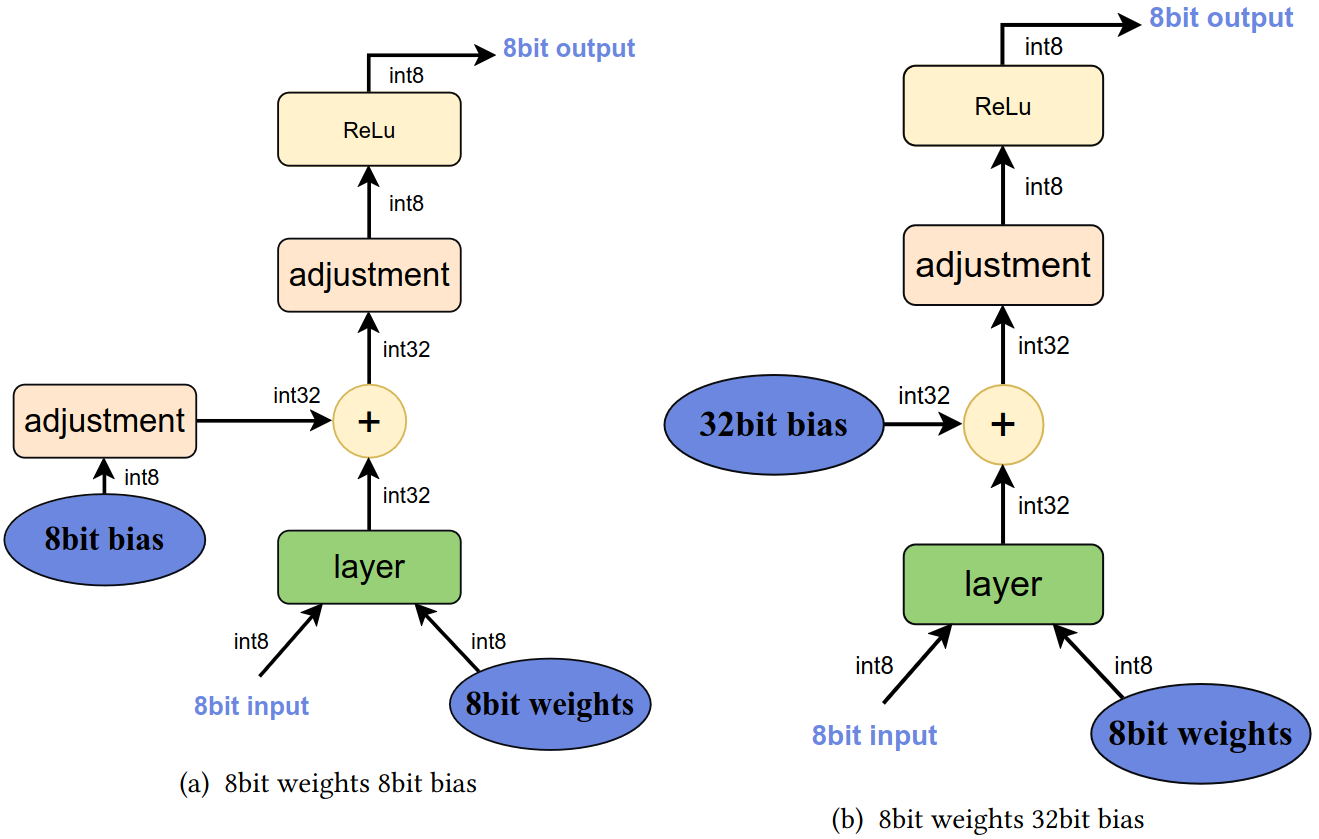
\includegraphics[width=0.8\textwidth]{figures/quant_schem_conv_layer.png}
\caption{Quantization schematic of a convolutional layer showing both 8-bit weights with 8-bit bias and 8-bit weights with 32-bit bias}
\label{fig:convolutional_layer_combined}
\end{figure}

Figure~\ref{fig:convolutional_layer_combined} shows the quantization schematic of a convolutional layer with both 8-bit weights and biases, and 8-bit weights with 32-bit biases.

%%%

\subsection{Quantization Techniques in Neural Network Optimization}

In the optimization of neural networks for efficient deployment, two prominent quantization techniques are utilized: Quantization-Aware Training (QAT) and Post-Training Quantization (PTQ). 

\subsubsection{Quantization-Aware Training (QAT)}
QAT is an approach where the model is trained (or fine-tuned) with quantization in mind from the beginning. This means that during the training process, the quantization effects are simulated, and the model parameters are adjusted accordingly. The goal is to mitigate the accuracy loss typically associated with quantization. This is depicted in the left part of the provided figure.

\subsubsection{Post-Training Quantization (PTQ)}
PTQ, on the other hand, involves calibrating and quantizing a pre-trained model without retraining from scratch. The model is calibrated using a subset of the training data to compute the clipping ranges and the scaling factors necessary for quantization. This method is particularly advantageous when aiming to reduce the time and computational resources required for model deployment. The right part of the provided figure illustrates this process.\\

Our implementation, as discussed in the DFQ Quantize Bias Correction paper, adopts the PTQ method due to its efficiency and practicality in deploying neural networks with minimal performance degradation.

% Include the figure here
\begin{figure}[H]
\centering
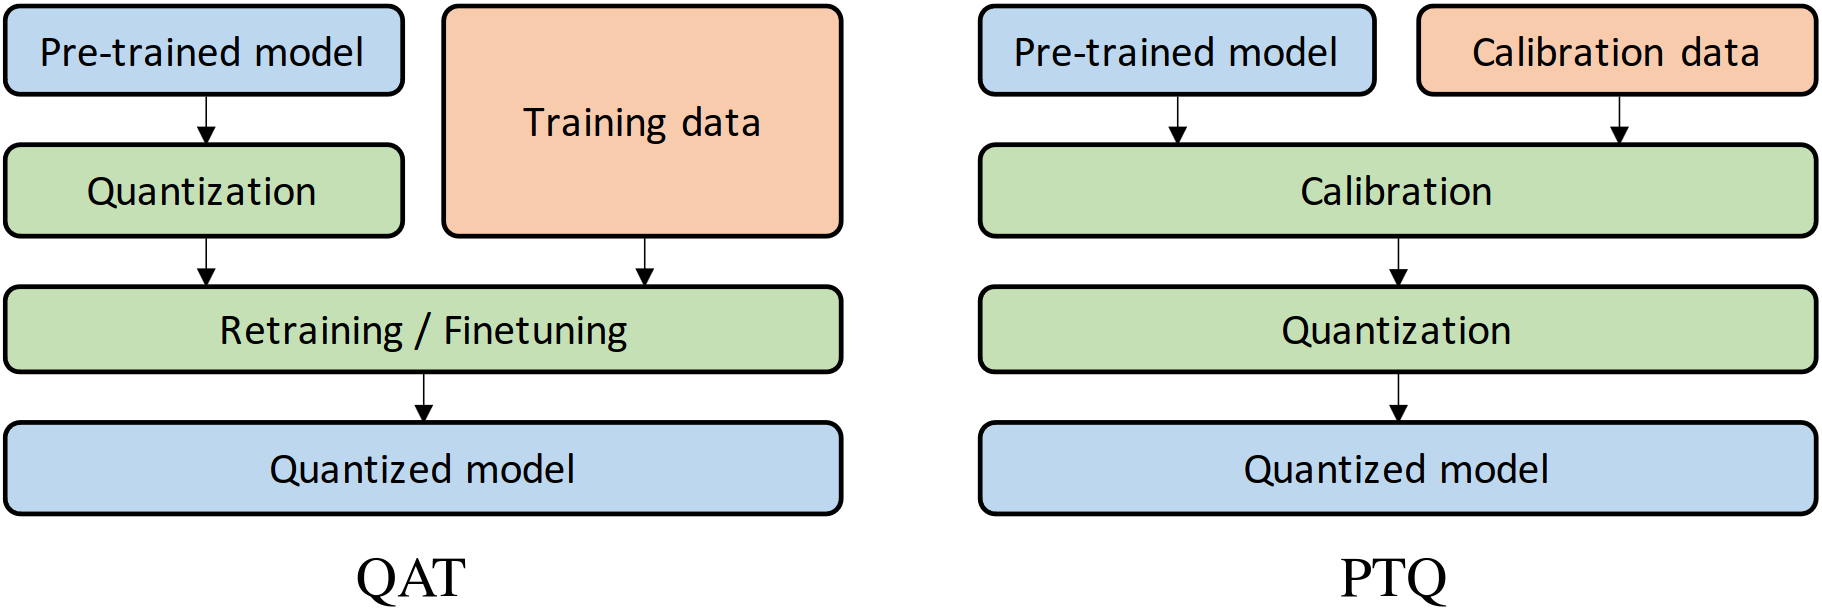
\includegraphics[width=\textwidth]{figures/qat_ptq.png}
\caption{Comparison of Quantization-Aware Training (QAT) and Post-Training Quantization (PTQ) methods.}
\label{fig:qat_ptq_comparison}
\end{figure}

As seen in Figure~\ref{fig:qat_ptq_comparison}, both QAT and PTQ are critical in the context of optimizing deep learning models for hardware efficiency. However, the choice between the two methods depends on the specific requirements and constraints of the deployment environment.

%%%



\subsection{Mathematical Formulation}
This section explores the mathematical underpinnings of quantization bias correction, detailing the correction of errors introduced during the quantization process.

\subsubsection{Error Formulation}
Consider a fully connected neural network layer with a weight matrix \( W \) and its quantized version \( \tilde{W} \), with input activations \( x \). The quantized output is given by:
\begin{equation}
    y_e = \tilde{W} x = y + \epsilon_x
\end{equation}
Here, \( \epsilon = \tilde{W} - W \) denotes the quantization error, and \( y \) is the pre-activation output of the original model.

\subsubsection{Bias Correction Using Batch Normalization}
To correct for the quantization-induced bias, we adjust the batch normalization parameters. The expected output \( i \), if non-zero, changes the mean of the output distribution, which is corrected by:
\begin{equation}
    E[y] = E[y_e] - E[\epsilon_x]
\end{equation}
This ensures the mean of each output unit remains unchanged after quantization.

\subsubsection{Empirical Quantization Bias Correction}
In the absence of batch normalization across all layers of a neural network, empirical quantization bias correction becomes essential. This method relies on a dataset to empirically determine the quantization-induced deviations in the pre-activation outputs. The steps are as follows:
\begin{enumerate}
    \item \textbf{Collect Pre-activation Means in FP32 Model:} Run a set of \( N \) examples through the original FP32 model. For each layer \( L \), collect the per-channel pre-activation means, denoted as \( E[y_L] \), where \( y_L \) represents the pre-activation output of layer \( L \) in the FP32 model.
    
    \item \textbf{Pre-activation Means in Quantized Model:} Process the same \( N \) examples through the quantized model. For each layer \( L \), record the per-channel pre-activation means, denoted as \( E[\tilde{y}_L] \), where \( \tilde{y}_L \) indicates the pre-activation output of layer \( L \) in the quantized model.

    \item \textbf{Compute Quantization Bias:} For each layer \( L \), calculate the per-channel biased quantization error \( E[\epsilon_L] \), where \( E[\epsilon_L] = E[\tilde{y}_L] - E[y_L] \). This quantifies the mean shift induced by quantization for each channel in layer \( L \).
\end{enumerate}

\subsubsection{Computing Expected Error}
The expected error \( E[\epsilon_x] \) is computed using the batch normalization layer's statistics, leveraging the scale (\( \gamma \)) and shift (\( \beta \)) parameters, particularly when activation functions such as ReLU are used. The expected value for a channel \( c \) post-activation is:
\begin{equation}
    E[x_c] = \gamma_c \cdot N\left(\frac{-\beta_c}{\gamma_c}\right) + \beta_c \cdot \left(1 - \Phi\left(\frac{-\beta_c}{\gamma_c}\right)\right)
\end{equation}
where \( N \) and \( \Phi \) represent the standard normal probability density function and cumulative distribution function, respectively.

\subsection{Understanding Bias Correction in Quantization}
Quantization often introduces a bias in error, which means there's a discrepancy between the expected output of the original and the quantized layer or network. This bias is particularly noticeable in depth-wise separable layers, where a limited number of weights per output channel (typically 9 for a 3×3 kernel) can lead to pronounced errors. Clipping error is a major contributor here, as a few extremely clipped outliers tend to shift the expected distribution.
\subsection{Addressing Bias through Layer’s Bias Parameter}
One effective method to counteract this bias is by adjusting the layer’s bias parameter. This adaptation helps in aligning the performance of the quantized model more closely with the original FP32 model's accuracy. The correction term, matching the shape of the layer bias, can be seamlessly integrated into the existing bias parameter, ensuring no additional overhead during inference.

\subsubsection{Methods of Bias Correction}

\paragraph{Empirical Bias Correction}
When a calibration dataset is available, the bias correction term can be calculated by comparing the activations between the quantized model and the full-precision model. This direct comparison allows for an empirical adjustment that enhances accuracy.

\paragraph{Analytical Bias Correction}
In the absence of calibration data, analytical methods, such as the one introduced by Nagel et al. (2019), can be employed. This approach utilizes batch normalization statistics from the preceding layer to estimate the expected input distribution, thereby analytically correcting for the biased error. This method is particularly applicable to networks with batch normalization and ReLU activations, offering a data-independent solution to bias correction.



%\subsection{Présentation de l'algorithme}
\subsection{Données}
\subsection{Evaluation expérimentale}

\subsection{Conclusion}

Post-training quantization emerges as a highly effective strategy for optimizing neural networks for hardware deployment, offering the advantage of reduced complexity without demanding extensive retraining periods. This technique is particularly adept at adapting models for 8-bit architectures, striking a balance between computational efficiency and model performance. However, as we venture into the realm of lower precision quantizations, such as 4-bit or even lower, the challenges become more pronounced.\\

When the precision drops to 4-bit or below, standard quantization methods may not suffice to maintain accuracy. This reduction in bit-depth leads to a significant loss of information, which can adversely affect the model's ability to make accurate predictions. To counteract this, advanced optimization techniques become indispensable. These may include employing more sophisticated quantization algorithms that are sensitive to the distribution of weights and activations, fine-tuning the model post-quantization, or utilizing mixed-precision techniques where different parts of the network are quantized to different extents.\\

Additionally, the choice of model architecture plays a crucial role. Some architectures are more resilient to quantization than others, and identifying or designing such models can be crucial for successful low-bit quantization. Networks with inherent redundancies or those designed with quantization in mind (quantization-aware training) tend to exhibit better tolerance to information loss due to lower precision.\\

In summary, while post-training quantization is a robust approach for preparing neural networks for efficient hardware implementation, especially at 8-bit precision, descending into lower bit-widths calls for a more tailored approach. It necessitates a combination of advanced quantization strategies, thoughtful model architecture choices, and potentially, some degree of retraining or fine-tuning to achieve the desired balance between efficiency and accuracy.

\end{document}

%% Le code de prof 
% INTRO section
\section{Introduction}
\label{sec:intro}

\textbf{L'introduction présente le contexte général lié à la tâche, description de la tâche à traiter, détail des problèmes qui y sont associés.} \\

\lipsum[2]

% METHODE section
\section{Présentation de l'algorithme}
\label{sec:methode}
\textbf{Une présentation synthétique de la solution ré-implémentée
de l’article. Précisez et justifiez les éventuelles
différences avec l'article de référence}\\

\lipsum[2]

% DATA section
\section{Données}
\label{sec:data}
\textbf{Présentation des bases de données utilisées. Précisez et justifiez les éventuelles différences avec l’article de référence.}\\

\lipsum[3]

% EXPERIMENT section
\section{Evaluation expérimentale}
\label{sec:experimence}


\subsection{Description de l'expérience}
 
\textbf{Description de l'expérience réalisée, méthodologie et métriques d'évaluation.} \\

\lipsum[4]

\subsection{Résultats}
 
\textbf{Présentation des résultats expérimentaux obtenus et  comparaison par rapport à ceux de l’article de réference.} \\

\lipsum[5]

\subsection{Discussion}

\textbf{Discussion critique à partir des
résultats obtenus} \\

\lipsum[6]




% CONCLUSION section
\section{Conclusion}
\label{sec:conclusion}

\textbf{Conclusion : un résumé synthétique des principaux résultat obtenus et présentation des principales pistes d'amélioration possibles.} \\

\lipsum[7]

% BIBLIO section
\section{Bibliographie}

\textbf{Bibliographie : une liste complète des principaux articles de l'état de l'art ou ayant inspiré la démarche, et qui seront référencés de manière pertinente dans le rapport.}\\

Par exemple \citep{Goodfellow-et-al-2016} et \citep{test}


\bibliography{biblio}



